\chapter{ILC Algorithms}
\label{ch:ILCAlg}

\newcommand{\IAgood}{30}
\newcommand{\IAbad}{50}
\newcommand{\badCondNb}{$1.353\, 10^{16}$}
\newcommand{\tol}{10^{-8}}



Imagine, that some action needs to be performed multiple times. 
For example, a robot manipulator must put objects in a box with high accuracy, while the objects to put are always located in the same place. It takes the same path again and again. If an input sequence for this issue solving already exists, it can be used for the next iteration and delivers the same precision. The other possibility is to ''learn'' from the previous iteration and try to enhance the exactness.




First, assume the system \eqref{eq:Basics:GP} to have stable matrix $A$. There is no less of generality, if the system is stabilizable. 
In this case, it is always possible to find such a matrix $F$, such that in the system 
\begin{align}
\begin{mtrx}{c}
x(t+1) \\ y(t)
\end{mtrx} = 
\begin{mtrx}{c c}
A - BF & B \\ C - DF & D
\end{mtrx}
\begin{mtrx}{c}
x(t) \\ v(t)
\end{mtrx}
\end{align}
the matrix $A - BF$ is stable. The new input is here given by $v:= u - B F x$. Depending on controller, there are other ways to transform the system, such a new input is defined, which can be adjusted using ILC algorithms. An example for a system controlled by a controller based on separation principle is presented below. 


\begin{exam}
\label{ex:ILC:LQR}
Consider a stabilizable and detectable system $(A,B,C,D)$ with input $u$ and output $y$. 
Extend the input $u$ to $u + \t u$, where $u$ is controlled with controller based on separation principle $u(t) = -F \hat x(t) + M r(t)$, $t \geq 0$, and $\t u$ is initially zero. Then the system can be rewritten as
\begin{align}
x(t+1) & = (A - BF)x(t) + B(F \t x(t) + \t u(t) + M r(t)), \\
y(t) & = (C - DF)x(t) + D(F \t x(t) + \t u(t) + M r(t)), \;\; t \geq 0.
\end{align}
This system is stable. Defining $v(t):=F \t x(t) + \t u(t) + M r(t)$, $t \geq 0$, this system can be used for ILC algorithms, while the initial input is 
\begin{align}
v_0 = \begin{pmatrix}
M r(0) \\ F \t x(1) + M r(1) \\ F (A - JC) x(1) + M r(2)\\ \vdots \\ F(A - JC)^{N-2} x(1) + M r(N)
\end{pmatrix}.
\end{align}
\end{exam}

\begin{exam}
	
	
	Consider the system $(A,B,C,D)$ with 
	\begin{align}
	\label{eq:ILC:Sys_ex1}
	A = \begin{pmatrix}
	2 & 1 \\  4 & 3
	\end{pmatrix}, B = \begin{pmatrix}
	1 \\ 2
	\end{pmatrix}, C = \begin{pmatrix}
	0 & 1
	\end{pmatrix}, D = 2.
	\end{align}
	
	
	This system is asymptotically stabilizable and detectable. Use the same notation as in Chapter \ref{ch:stabilizingController}, and choose the weights $Q = 3$ and $R = 2$. Then 
	\begin{align}
	F =\begin{pmatrix}
	1.9674  &  1.3042
	\end{pmatrix} \text{ and } 
	J = \begin{pmatrix}
	1.8705  &  4.7321
	\end{pmatrix}
	\end{align}
	can be used for the controller based on separation principle. 
	
	
	Then the system is modified to 
	\begin{align}
	\label{eq:ILC:Sys_ex1_modified}
	\begin{array}{c c c c c c c c c}
	x(t+1) &=&
	\begin{pmatrix}
	0.0326  & -0.3042\\
	0.0652  &  0.3916
	\end{pmatrix}
	& x(t) &+& 
	\begin{pmatrix}
	1 \\ 2
	\end{pmatrix}
	v(t)& &
	\\ 
	y(t)   &=& \begin{pmatrix}
	-3.9348  & -1.6084
	\end{pmatrix}
	& x(t)& +&
	2 v (t),& &\; t = 0, 1, 2, \dots, N
	\end{array}
	\end{align} with a new input signal $v(\cdot)$. 
	
\end{exam}

\section{Inverse Model Algorithms}

Consider again the equation \eqref{eq:Gu + d}. 
The tracking problem here seems to be straightforward.
If the reference signal $r$ is known, a perfect solution can be find by choosing 
\begin{align}
u_\infty = G^{-1} r -d.
\end{align}

However, this choice does not look greatly credible. 
For example, if a measurement are disturbed by noise, the output signal becomes
\begin{align}
y + \varepsilon w = G u_\infty + d + \varepsilon w = r + \varepsilon w \neq r,
\end{align}
for some non-zero vector $w \in \R^{m(N+1)}$ and a small $\varepsilon > 0$. 
Also for uncertain models this method might not be applicable, as it can be difficult to calculate the inverse. 
This idea can be reformulated in a more robust way, and result in a good and simple applicable algorithm, which is called the \textit{Inverse Model Algorithm.}


\begin{alg}
	\label{alg:ILC:IA}
	Let the matrix $D$ in \eqref{eq:Basics:GP} be square (i.e. $m = l$) and invertable. Then the matrix $G = G(A, B, C, D)$ is non-singular as well, and the Inverse Model Algorithm (IA) is given via input update law 
	\begin{align}
	\label{eq:errRightInv}
	\begin{split}
	u_{k+1} &= u_k + \beta G^{-1} e_k, \\
	u_0 & \in \R^{m (N+1)}.
	\end{split}	
	\end{align}
	The error evolution follows
	\begin{align}
	\label{eq:Alg:e_k+1 = (1 - beta) e_k}
	\begin{split}
	e_{k+1} &= (1- \beta) e_{k}, \; k\geq 0, \\
	e_0 &= r -  Gu_0 -d.
	\end{split}
	\end{align}
	In particular, $(e_k)_{k\geq 0}$ converges to zero for $k \to \infty$ for any initial error $e_0 \in \R^{m(N+1)}$ if and only if 
	\begin{align*}
	0 < \beta < 2.
	\end{align*}
\end{alg}
\begin{proof}
	Firstly, the matrix $G\in \R^{(N+1)m \times (N+1) m}$ is also square and has the lower triangular structure, with the matrix $D$ on its diagonal. Hence, $\det(G) = \det(D)^{N+1}$, which is non-zero if and only if $D$ is invertable.
	Taking the limit over relation \eqref{eq:Alg:e_k+1 = (1 - beta) e_k} results in
	\begin{align}
	\lim_{k \to \infty} e_{k+1} = \lim_{k \to \infty}(1- \beta) e_{k} = \lim_{k \to \infty}(1 - \beta)^k e_0.
	\end{align}
	Choosing $0<\beta < 2$ yields the proof. 
\end{proof}

The choice of $\beta$ close to 0 or 2 yields slower convergence and better robustness. For $\beta = 1$ the algorithm converges in one iteration, but this choice might be non-robust \cite[pp 149, 152-155]{ILC}, .

An example of applying of this algorithm on the system \ref{eq:ILC:Sys_ex1_modified} is presented below. 

\begin{exam}
	\label{ex:ILC:badIA}
	In the system \eqref{eq:ILC:Sys_ex1_modified} the matrix $D = 2$ is invertible, and IA can be applied.  Choose $\beta = 0.1$. Convergence to 0 with tolerance $10^{-8}$ is achieved after 74 iterations.The result is illustrated in Figure \ref{img:ILC:Ex1_IA}.
			
	\begin{figure}[t]
		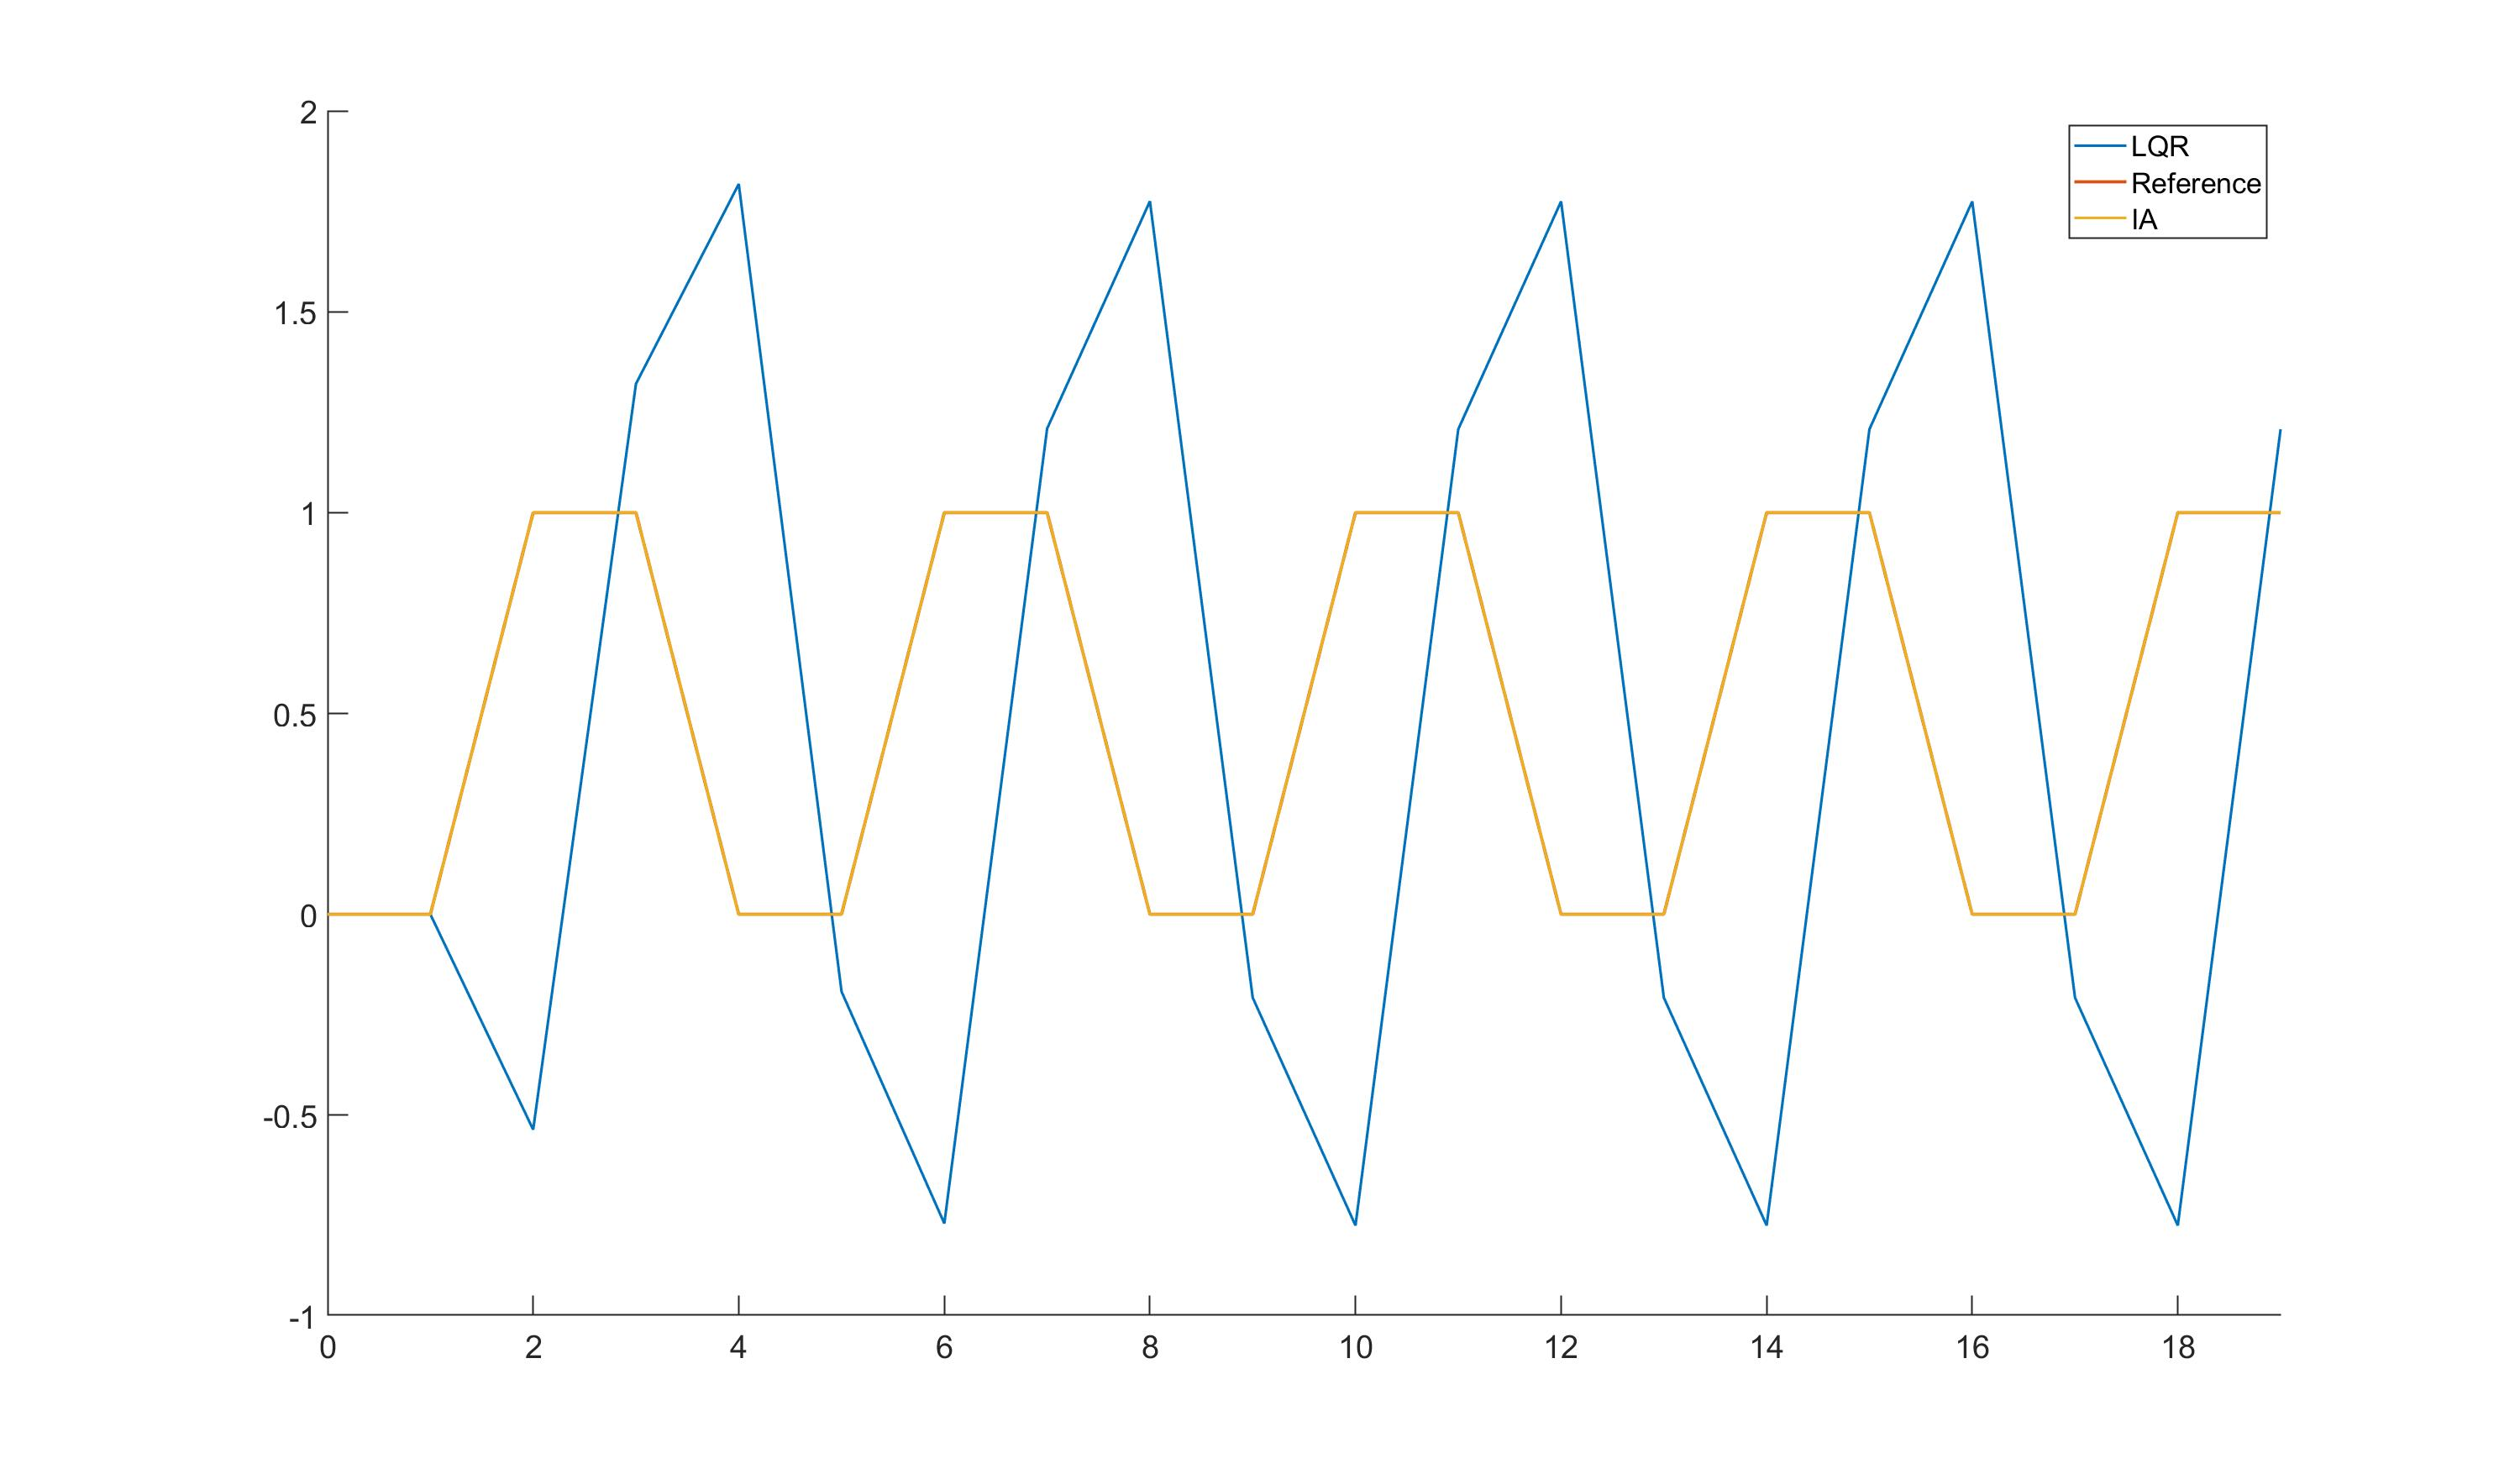
\includegraphics[width=\textwidth]{fig/Ex1_IA.jpg}
		\caption{Tracking with LQR Controller (without ILC algorithm), and tracking with IA for the system \eqref{eq:ILC:Sys_ex1} for $N = \IAgood$} 		\label{img:ILC:Ex1_IA}
	\end{figure}

	However, by trying to increase the length of the time horizon $N$, for example to {\IAbad} steps, the system behaviour is wrong  (Figure \ref{img:ILC:Ex1_IAbad}). 
		
			\begin{figure}[t]
			\centering
			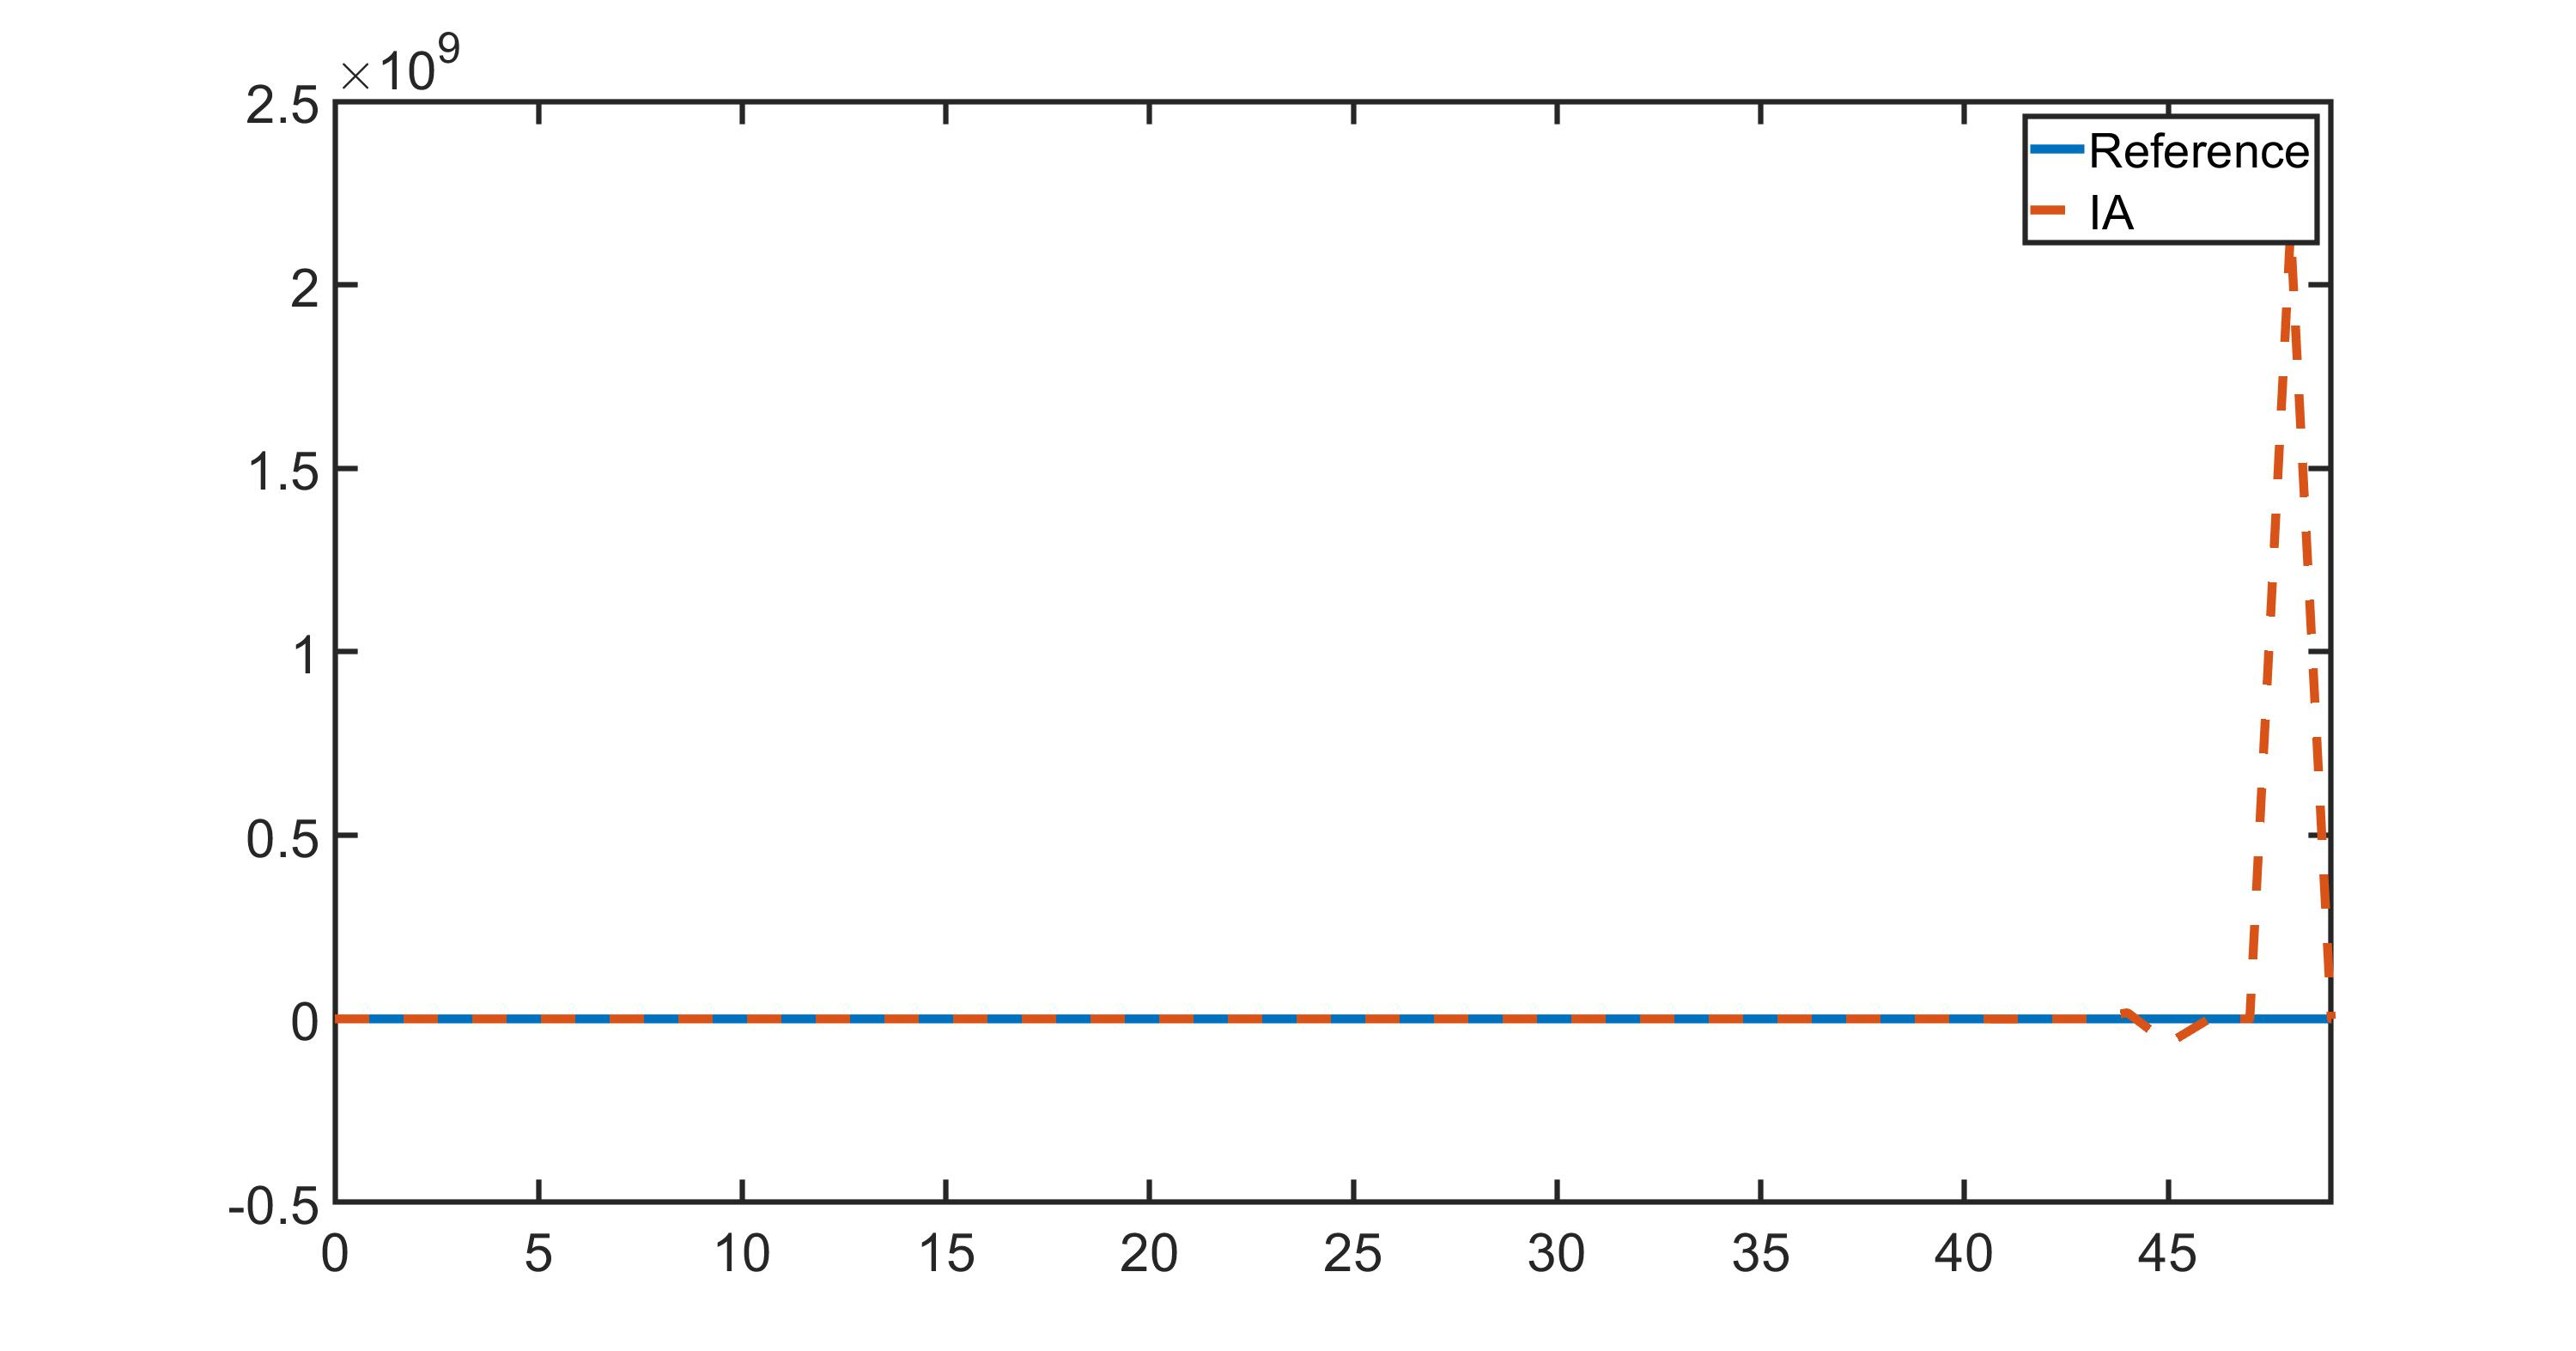
\includegraphics[width=\textwidth]{fig/Ex1_IAbad.jpg}
			\caption{Tracking with IA for the system \eqref{eq:ILC:Sys_ex1} for $N = \IAbad$}
			\label{img:ILC:Ex1_IAbad}
		\end{figure}
	
	The reason is the condition number of the matrix $G$, which equals \badCondNb. This shows: even for a triangular matrix with non-zero eigenvalues, the numerically disturbances can lead to an unexpected algorithm behaviour. 
		
\end{exam}

The Inverse Model Algorithm sets up very strong requirements: the matrix $G$ should be non-singular, and its condition number must be small enough, such that a an inverse can be correct computed by numerical methods. 
That motivates not to use the inverse of the matrix, but a pseudo-inverse. This is a uniquely defined matrix, which can be computed for any matrix, even not for a square one.

\begin{defi}
	\label{def:ILC:pseudoinv}
	For a matrix $G \in \R^{m(N+1) \times l(N+1)}$ a psedo inverse is defined by a matrix $G^+ \in \R^{l(N+1) \times m(N+1)}$, satisfying the criteria: 
	\begin{enumerate}
		\item $G G^+ G  = G $,
		\item $G^+ G G^+ = G^+$,
		\item $(G G^+)^T = G G^+$,
		\item $(G^+ G)^T = G^+ G$.
	\end{enumerate}
\end{defi}


\begin{alg}
	\label{alg:ILC:PIA}

	The Pseudo Inverse Model Algorithm (PIA) is given via input update law 
	\begin{align}
	\label{eq:ILD:errPIA}
	\begin{split}
	u_{k+1} &= u_k + \beta G^{+} e_k, \\
	u_0 & \in \R^{l (N+1)},
	\end{split}	
	\end{align}
	with  the error evolution
	\begin{align}
	\begin{split}
	e_{k+1} &= (I- \beta G G^+) e_{k}, \; k\geq 0, \\
	e_0 &= r -  Gu_0 -d.
	\end{split}
	\end{align}

	Monotonic convergence to 
	\begin{align}
	\label{eq:ILC:einfPIA} 
	e_\infty  = \lim_{k\to\infty} e_k = P_{\ker[G^+]}e_0,
	\end{align} 
	is guaranteed if
	\begin{align*}
	0 <\beta < 2.
	\end{align*}
	$P_{\ker[G^+]}$ denotes the positive orthogonal projection operator onto $\ker[G^+]$.
	In particular, the zero convergence is attainable, if and only if the tracking signal $r$ is feasible. That is, there exists an input $u_\infty$, such that $r = G u_\infty + d$. %$e_0 \in \im [G G^\star]$. 
\end{alg}
\begin{proof}
	Because of the pseudo inverse definition, it holds
	$(GG^+)^2 = GG^+GG^+ = GG^+$.  Then the error evolution formula can be proven by mathematical induction over $k$. 
	
	For $k = 1$ it follows: 
	\begin{align*}
	e_1 = (I - \beta G G^+)e_0 = (I + GG^+ - GG^+ - \beta G G^+)e_0 = (I + \left[(1 - \beta) + 1\right]GG^+)e_0.
	\end{align*}
	
	For $k \in \N$  
	\begin{align*}
	e_{k+1} &= ( I - \beta G G^+)e_k = ( I - \beta G G^+) (I+  \left[(1-\beta)^{k-1} - 1\right] G G^+) e_0 = \\
	& = \left(I - \beta G G^+ + (1-\beta)^{k-1}GG^+ - GG^+ - \beta GG^+\left[(1 - \beta)^{k-1} - 1\right]GG^+\right)e_0=\\
	& = \left(I - (\beta - (1-\beta)^{k-1} + \beta\left[(1 - \beta)^{k-1} - 1\right])G G^+\right)e_0\\
	& = \left(I - \left(\beta - (1-\beta)^{k-1} + 1 + \beta(1-\beta)^{k-1} - \beta\right)GG^+\right)e_0\\
	& = (I+  \left[(1-\beta)^k - 1\right] G G^+) e_0
	\end{align*}
	         
	To prove \eqref{eq:ILC:einfPIA}  recall that 
	\begin{align*}
	\R^{m(N+1)} = \im(G)\oplus \ker (G^+),
	\end{align*}
	The symbol $\oplus$ denotes here the direct sum of two vector spaces. %TODO: Laag als Quelle 
	Hence, $e_0$ can be written as 
	\begin{align*}  
	e_0 = G w_0 + v_0,
	\end{align*}
	where $v_0 = (I - G G^+)e_0 \in \ker (G^+)$  is uniquely defined and $w_0 = G^+ e_0 \in \R^{l(N+1)}$. It follows: 
	\begin{align*}
	e_{k} = (1+ \left[(1 - \beta)^{k-1} - 1\right]GG^+)e_0 = (1-\beta)^{k-1} G w_0 + v_0.
	\end{align*}
	For $\beta \in (0,2)$ the error $e_k$ converges to $v_0$ for $k \to \infty$. 
	
	
	Further, it is clear, that if the error $e_k$ converges to zero, the problem is feasible with $u_\infty = \lim_{\k} u_k$. On the other hand, if the problem is feasible, it holds
	\begin{align}
	e_k = r - y_k = G(u_\infty - u_k), 
	\end{align}
	and hence by using the property (a) from Definition \ref{def:ILC:pseudoinv}
	\begin{subequations}
	\begin{align}
	e_{k+1} &= (I- \beta G G^+) e_k = (I- \beta G G^+) G(u_\infty - u_k)
	\\
	&= (G - \beta G G^+ G)(u_\infty - u_k) = (1 - \beta)G(u_\infty - u_k) 
	\\
	&= (1- \beta) e_k = (1 - \beta)^k e_0 \to 0 \text{ as } k \to \infty,
	\end{align}
	\end{subequations}
	because of choice of $\beta$. 
\end{proof}

\begin{exam}
	\label{ex:ILC:PIA}
	Calculate a solution for \eqref{eq:ILC:Sys_ex1} with PIA, and illustrate it in Figure \ref{fig:ILC:Ex1_PIA}. 	
	This time the tracking signal and system output fit well despite the large condition number. However, a deviation can be observed at the beginning, which causes the bad invertability of the matrix $G$. 
	  
	\begin{figure}[ht!]
		\centering
		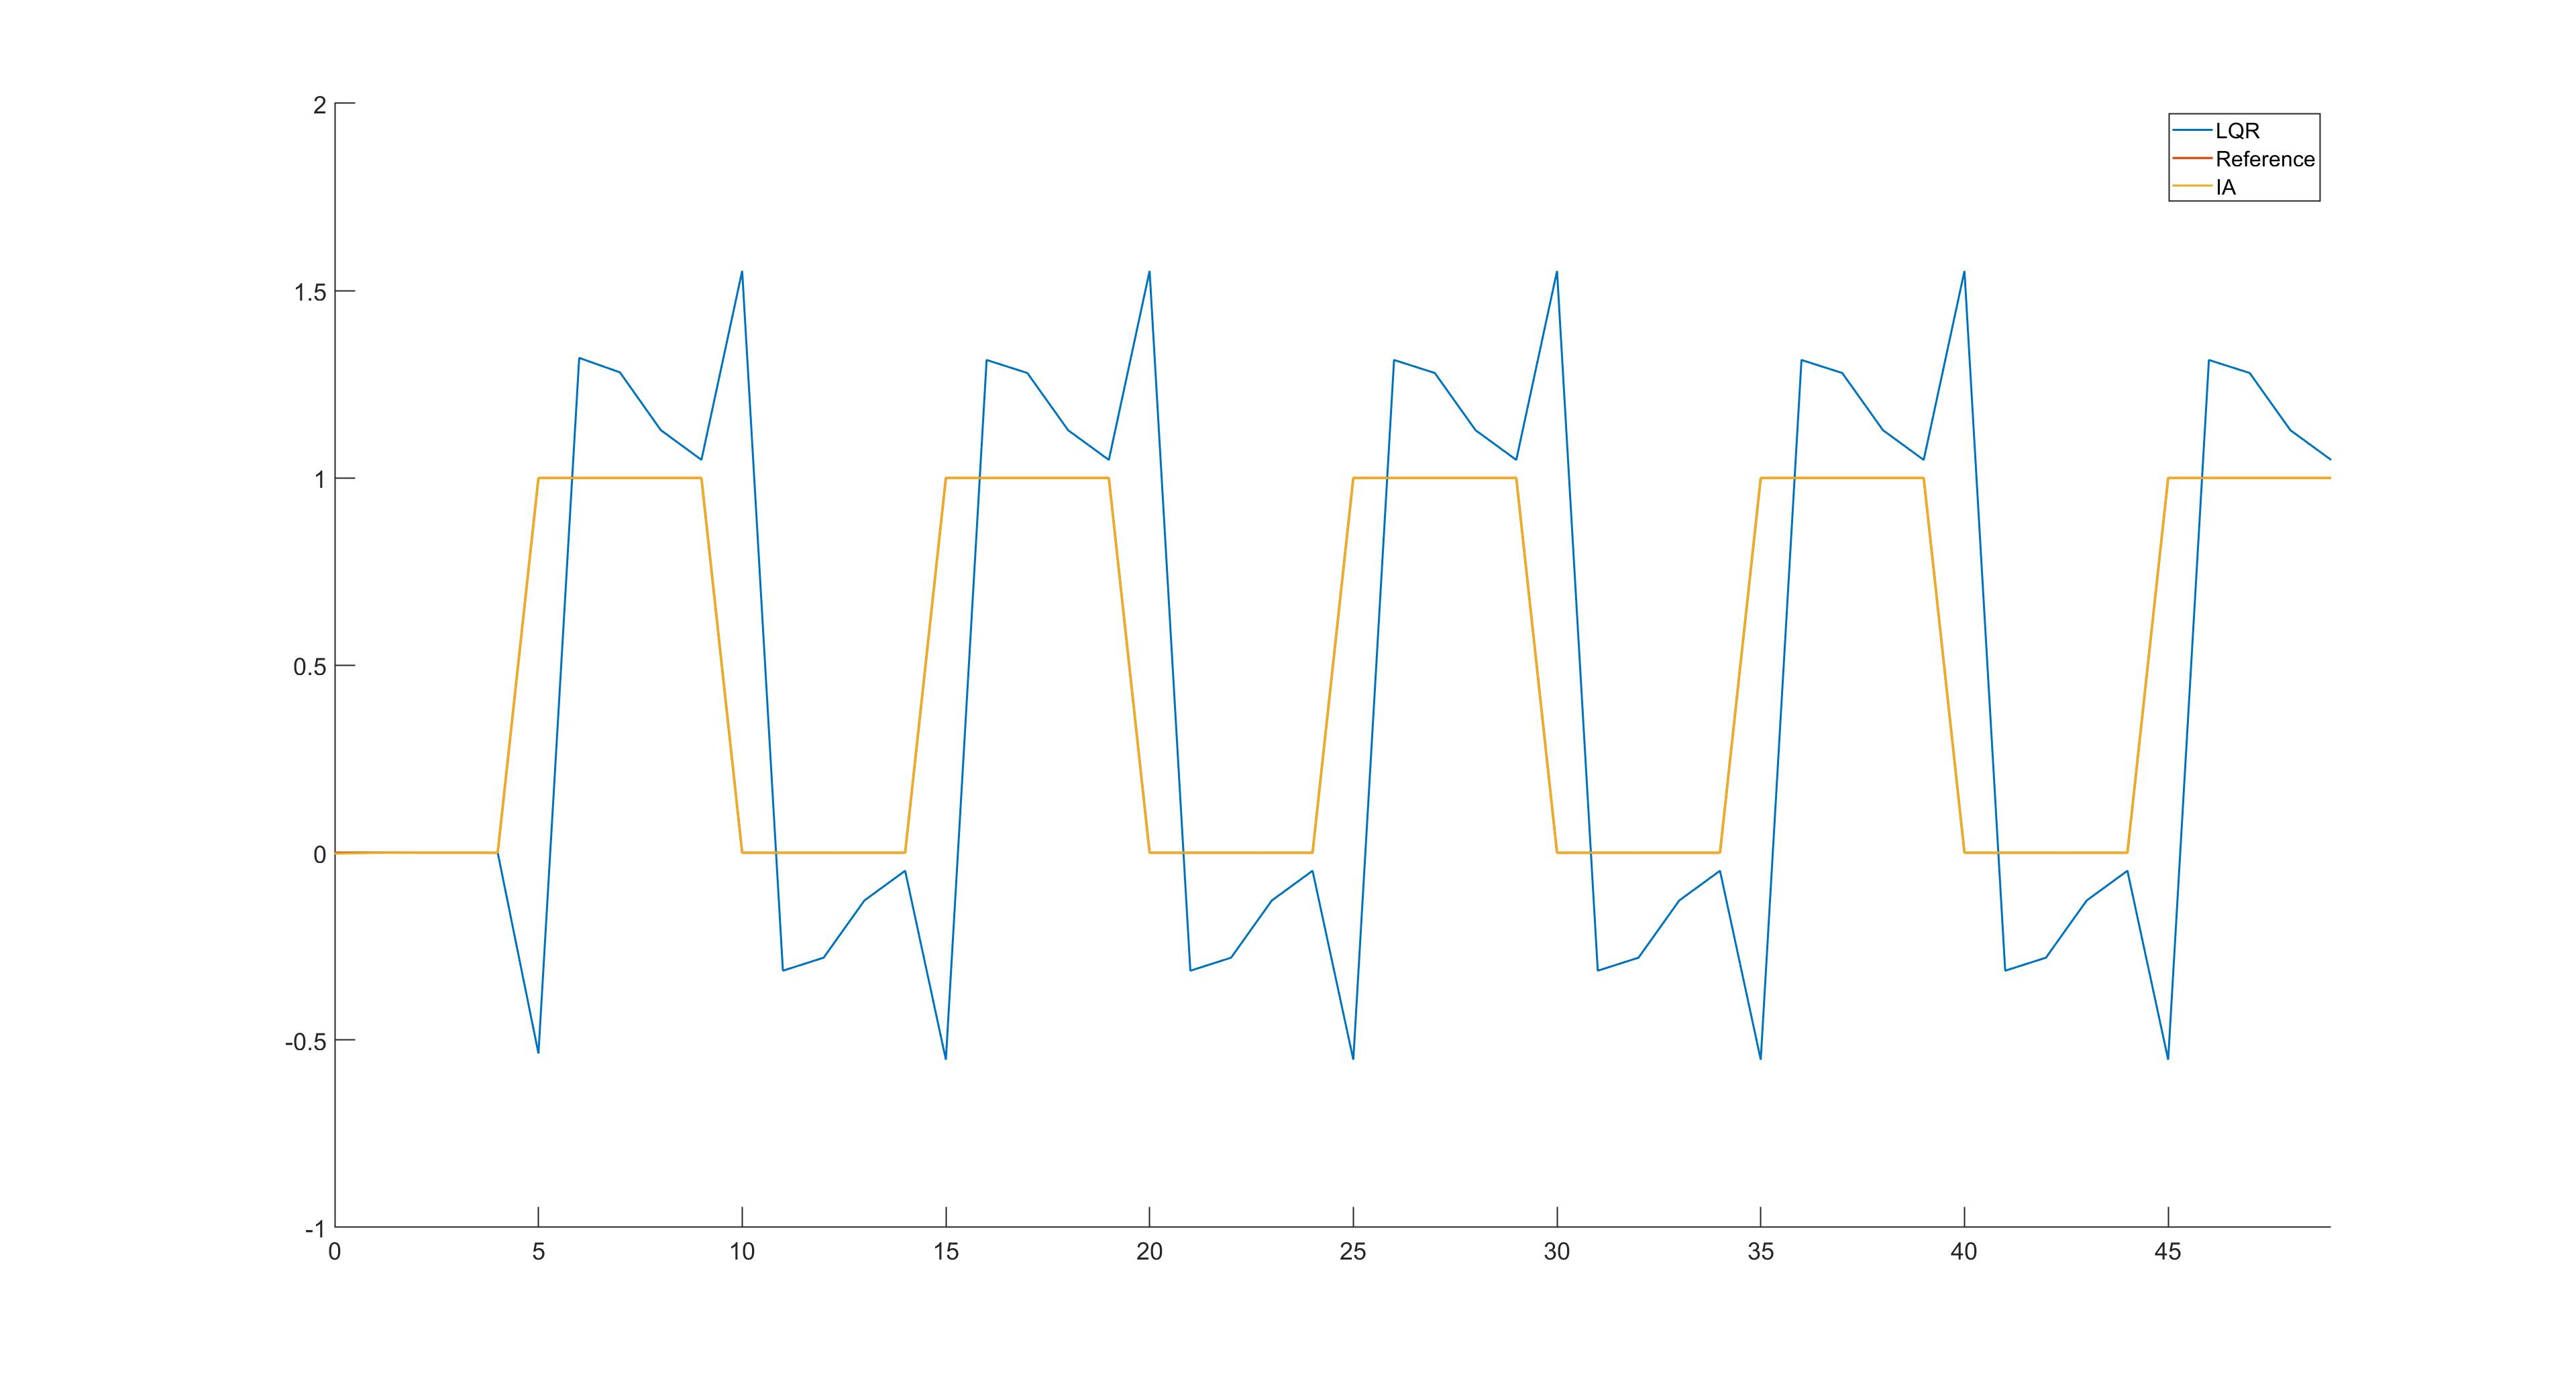
\includegraphics[width=\textwidth]{fig/Ex1_PIA.jpg}
		\caption{Reference signal tracking with LQR and PIA for the sysytem \eqref{eq:ILC:Sys_ex1} for $N = \IAbad$ }
		\label{fig:ILC:Ex1_PIA}
	\end{figure}
\end{exam}


Owens in his book \cite{ILC} chooses the left and right inverse matrix instead of the pseudo inverse. 
The pseudo inverse has its advantage to equal the right/left inverse, if it exists. Moreover, for right/left inverse does not exist for any matrix. 
The algorithm in the above presented formulation can be applied for any matrix $G$ and can be linked to the feasibility of the tracking value $r$. 
 	
The Algorithm \ref{alg:ILC:IA} is a special case of PIA. However, numerically the use of the inverse matrix might be more desirable as it requires less calculation effort, if the condition number is not large. 

The (Pseudo) Inverse Algorithm belongs to the class of so-called Unit Memory Algorithms. These are the algorithms which can  ''remember'' the last trial. 

\section{Unit Memory Algorithms}

Of interest are the processes, which are executed repetitively. Let $k = 0, \, 1, \, 2, \, \dots $ be the number of completed iterations. Then for the $k$-th trial the system, it holds
\begin{align}
\label{eq:unitMemory}
\begin{split}
y_{k} &= G u_k + d,  \\ %& &\text{ (The Input Update Rule)} 
e_k &= r - y_k, 
\end{split}
\end{align}
with some initial input $u_{0} \in \R^{l(N+1)}$. 
%This is again a discrete-time system, with time increment $k$. 

%the monotonic convergence to some $e_\infty \in \R^{m(N+1)}$ is desirable :
%\begin{align}
%\lim_{k \to \infty} e_k = e_\infty, \text{ and } ||e_{k+1} || \leq ||e_k|| \text{ for all } k \geq 0.
%\end{align}

%First we try to formulate an iteration law for the input signal, and calculate then the error sequence as 
%\begin{align}
%e_k = r - y_k = r - G u_k - d, k \geq 0.
%\end{align}

Each pass $k$ the tracking can be improved, if the update law is chosen properly. Assuming the linear dependency of $u_{k+1}$ upon $u_k$ and $e_k$ for $k \geq 0$, the following algorithms results by using the feedback control. 
\begin{alg}
	\label{alg: unitMemory}
	The Unit Memory Algorithm is given via the input update law 
	\begin{align}
	\label{eq:clPlant}
	\begin{split}
	u_{k+1} &= u_k + K e_k, \\
	& u_0 \in \R^{l (N+1)}.
	\end{split}
	\end{align}	 
	The error dynamic is then given via
	\begin{align}
	e _{k+1} &= (I - G K) e_{k}, \; k \geq 0,\\
	e_0 &= r -  Gu_0 -d.
	\end{align}
%	since 
%	\begin{align}
%	\begin{split}
%	e_{k+1} &=  r - y_{k+1} = r - G u_{k+1} - d =\\
%	&= r - Gu_k - G Ke_k - d = e_k - G Ke_k, \; k\geq0.
%	\end{split}
%	\end{align}
	$K \in \R^{l(N+1) \times m(N+1)}$ is called \textbf{learning matrix}. 
\end{alg}


To achieve a good tracking at trial $k$ the norm $||e_k||$ is must be small. 
The tracking behaviour improves for consecutive iterations if the sequence $||e_k||$ is monotonically decreasing, i.e., 
\begin{align}
\label{eq:ILC:monotonisity}
||e_{k+1} || < ||e_k|| \text{ for all } k \geq 0.
\end{align}
Note that in this case the sequence $||e_k||$ is guaranteed to converge. If the sequence even converges to zero, the perfect tracking is achieved asymptotically.

To the small error, it is enough to consider the iteration process 
\begin{align}
\label{eq:e_k}
e_{k+1} = (I - G K) e_k = (I - G K)^k e_0  : =  L^k e_{0}, \; k \geq 0.
\end{align}

This is a discrete time dynamical system over $k$. Then the goal can be reformulated as follows: find some matrix $K \in \R^{l(N+1) \times m (N+1)}$, which renders \eqref{eq:e_k} stable. %In other words, we are looking for a stabilizing controller $K$. 

Rewriting the system as
\begin{align}
\label{eq:ILC:e_kPlant}
\begin{pmatrix}
e_{k+1} \\ e_k
\end{pmatrix} = 
\left(
\begin{array}{c|c}
I & -G \\\hline I & 0
\end{array}\right) \begin{pmatrix}
e_k \\ v_k 
\end{pmatrix},
\end{align}
our problem reduces to finding a stabilizing controller $K$  with 
\begin{align}
v_k = K e_k.
\end{align} 

At the beginning of this thesis one way to calculate such a controller was presented: the controller based on separation principle. This is a reliable method, but since the matrix $G$ can have a 	large dimension, it also can be costly. Often good results are achievable with more simple methods. For example, the number of parameters to be chosen can be reduced. 
In the presented Algorithms \ref{alg:ILC:IA} and \ref{alg:ILC:PIA}, the number of parameters to be chosen was reduced to 1, and these algorithms still show acceptable results. With notation from Algorithm \ref{alg: unitMemory}, the Algorithms \ref{alg:ILC:IA} and  \ref{alg:ILC:PIA} can be written as 
\begin{align}
K = \beta K_0
\end{align}
with a fixed matrix $K_0$ as the (pseudo) inverse of $G$, and left the parameter $\beta$ to decide on. 



However, the calculation of the  inverse matrix can be not very reliable method. The pseudo inverse delivers better results, but is also much more expensive. 
An algorithm, which does not require the model inversion, might be of use here. 
			
\section{Gradient Algorithms}
The aim of the ILC algorithms is to make the error $||e_k||$ small in some norm $||\cdot||$ in $\R^{m(N+1)}$. It is advantages, even to have a monotonic convergence, which means the \eqref{eq:ILC:monotonisity} must hold. In the above algorithms, the straightforward way was used: some algorithm was chosen based on the system, and the error norm was shown to converge to some $e_\infty \in \R^{m(N+1)}$. Now, derivate an algorithm from the other side, and begin with the consideration of the error norm in the first place. 


Choose the norm by defining the weighting matrices  $Q(t)$ and $R(t)$, $t = 0, 1, 2, \dots ,N$. Let the norms $||\cdot||_Q$, $||\cdot||_R$ to be defined associated with scalar products 
\begin{align}
\label{eq:SkPrQR}
\langle y,z\rangle_Q = \sum_{t = 0}^N y(t)^TQ(t)z(t), \; \langle u,v\rangle_R = \sum_{t = 0}^N u(t)^T R(t) v(t),
\end{align}
with $y(t), z(t) \in \R^{m}$, $u(t), v(t) \in \R^l$ for $t = 0,1,2, \dots, N$.
Furthermore, define the matrix 
\begin{align}
G^\star &= R^{-1} G^T Q \text{ for all } G \in \R^{m(N+1)\times l(N+1)},
%\\ K^\star &= Q^{-1} K^T R \text{ for all } K \in \R^{l(N+1)\times m(N+1)},
\end{align}
where 
\begin{align}
	\begin{split}
	Q :=& \diag(Q(0), Q(1), Q(2) ,\dots, Q(N)) \text{ and } \\
	R:=& \diag(R(0), R(1), R(2), \dots, R(N)).
	\end{split}
\end{align}



Recall, that for $R = I$ and $Q = I$ the matrices $G^\star$ and $K^\star$ are just the conjugate transpose. The notation from above can be seen as conjugate transpose in the vector space with scalar products \eqref{eq:SkPrQR}.

Applying the weighted norms on \eqref{eq:ILC:monotonisity} provides
\begin{align}
\begin{split}
||e_{k+1} ||_Q^2 &= ||e_k - G K e_k||_Q^2 = ||e_k||_Q - 2\langle e_k , G K e_k \rangle_Q + ||G K e_k||_Q^2 \\ 
&< ||e_k||_Q^2, \text{ if } ||GK e_k||_Q^2 < 2 \langle e_k, GK e_k\rangle_Q. 
\end{split}
\end{align}

The last inequality is equivalent to 
\begin{align}
e_k^T K^T G^T Q GK e_k < 2 e_k^T Q GK e_k.
\end{align}

If $K = \beta G^{\star}$, this is implicated by 
\begin{align}
\label{eq:ILC:SDA_Herleitung}
\beta^2 (G G^{\star})^T Q (G G^{\star}) \prec \beta Q G G^{\star} + \beta (Q G G^{\star})^T.
\end{align}

Since the matrix $Q$ is positive definite, there exists a positive definite matrix $Q^{1/2}$, such that $Q = Q^{1/2}Q^{1/2}$. 

Write $Q^{-1/2}$ for $\left(Q^{1/2}\right)^{-1}$, and define a matrix 
\begin{align}
H :=  Q^{1/2} G G^\star Q^{-1/2}. 
\end{align}
The matrix $H$ has the same eigenvalues as $G G^{\star}$, as for its characteristic polynomial holds 
\begin{align}
\label{eq:ILC:determinantGH}
\begin{split}
\det (I - \lambda H) &= \det \left(I - \lambda Q^{1/2} G G^\star Q^{-1/2}\right) \\
&= \det\left(Q^{1/2}\right)\det\left(I - \lambda G G^\star\right) \det\left(Q^{1/2}\right)^{-1} \\
&= \det\left(I - \lambda G G^\star\right) \text{ for any } \lambda \in \R. 
\end{split}
\end{align}

Rewrite \eqref{eq:ILC:SDA_Herleitung} as 
\begin{align}
\beta^2 H^T H \prec \beta (H + H^T). 
\end{align}

This relation is fulfilled if 
\begin{align}
0 < \beta < \frac{2}{\lama(H)}, 
\end{align}
where $\lama(H)$ is the greatest eigenvalue of the matrix $H$ in its absolute value. 


This deliberation inspires the \textit{Steepest Descent Algorithm}. 

\subsection{Steepest Descent Algorithm}
\begin{alg}
	\label{alg:SDA}
	The Steepest Descent Algorithm is characterized by choosing $K = \beta G^\star$, where $\beta>0$ is a real scalar gain. The input update law is given via 
	\begin{align}
	\label{eq:errSDA}
	\begin{split}
	u_{k+1} &= u_k + \beta G^\star e_k,\\
	u_0 &\in \R^{l (N+1)}, 
	\end{split}
	\end{align}
	and error evolution results in 
	\begin{align}
	e_{k+1} &= (I- \beta G G^\star) e_{k}, \; k\geq 0.
	\end{align}
	Monotonic convergence to 
	\begin{align}
	\label{eq:SDAErrLim} 
	e_\infty  = \lim_{k\to\infty} e_k = P_{\ker[G^\star]}e_0,
	\end{align} 
	is guaranteed if
	\begin{align*}
	0 <\beta < \frac{2}{\lama(H)}.
	\end{align*}
	Convergence to zero is assured in the case that $e_0 \in \im [G G^\star]$ holds.
\end{alg} 
\begin{proof}

To prove the statement remember that, as $GG^\star$ is a symmetric matrix. This implies a bunch of useful properties. 
Firstly, there exit the unique vectors 
$e_{\im} \in \im(G G^\star)$, $e_{\ker} \in \ker(G G^\star)$, such that 
\begin{align}
e_0 = e_{\im} + e_{\ker}.
\end{align}


Substituting $e_0$ in error evolution by this expression results in
\begin{align}
\label{eq:ILC:SDAerrorproof}
e_{k+1} = (I - \beta G G^\star) e_k = (I - \beta G G^\star)^k e_{\im} + e_{\ker}.
\end{align}

Furthermore, there exist an invertable matrix $S \in \R^{m (N+1) \times m (N+1)}$ and a diagonal matrix $\Lambda  =\begin{pmatrix}
\lambda_1 & & & \\ & \lambda_2 & & \\ & & \ddots & \\ & & & \lambda_{m(N+1)}\end{pmatrix}$, such that $(I - \beta G G^\star) = S^{-1}\Lambda S$. The values $\lambda_i$, $i = 1,2,\dots,\lambda_{m(N+1)}$ are the eigenvalues of the matrix 
$(I - G G^\star)$. 

Then \eqref{eq:ILC:SDAerrorproof} becomes 
\begin{subequations}
	\begin{align}
e_{k+1} &= (I - \beta S^{-1}\Lambda S)^k \, e_{\im} + e_{\ker} =  S^{-1}(I - \beta \Lambda)^k S \, e_{\im} + e_{\ker} 
\\
&= S^{-1}
\begin{pmatrix}
1 - \beta \lambda_1 & & & \\
& 1 - \beta \lambda_2 & & \\
& & \ddots & \\
& & & 1 - \beta \lambda_{m(N+1)}
\end{pmatrix}^k
 S \, e_{\im} + e_{\ker} 
 \\
 &= S^{-1}
 \begin{pmatrix}
 (1 - \beta \lambda_1)^k & & & \\
 & (1 - \beta \lambda_2)^k & & \\
 & & \ddots & \\
 & & & (1 - \beta \lambda_{m(N+1)})^k
 \end{pmatrix}
 S \, e_{\im} + e_{\ker}.
\end{align}
\end{subequations}

Therefore, the $(I - \beta G G^\star)^k$ converges to 0 (and hence $e_k$ to $e_{\im}$) as $k \to \infty$, if and only if
\begin{align}
|1 - \beta \lambda_i|<1 \text{ for all } i = 1,2, \dots, m(N+1).
\end{align}
By using \eqref{eq:ILC:determinantGH}, the last statement becomes 
\begin{align}
|1 - \beta \lama(H)|<1. 
\end{align}

This yields the proof. 
\end{proof}



An interesting observation is, that provided by this algorithm signal $u_\infty$ is the unique solution of the (minimum norm) optimization problem 
\begin{align}
u_\infty = \arg \min_{u \in \R^l(N+1)} \{|| u - u_0||_R^2: \text{ subject to } r = Gu + d\}.
\end{align}
One consequence is that the choice of $u_0$ has more significance than the simple intuition. A good choice will influence convergence rates beneficially. More generally, the limit $u_\infty$ is the closest input to $u_0$ in the norm, and since choosing $u_0 = 0$ leads to the minimum energy solution $u_\infty$ \cite[p.\~ 168]{ILC} p. 168. 

\leer


\textbf{Choice of the Weighting Matrices}

The choice of the weighting matrices $Q$ and $R$ provides the additional degrees of freedom. 
It impacts the behaviour of the algorithm. For example, with the choice of the matrix $Q$, some elements of input and output signals can be weighted, depending on their importance in measuring accuracies and convergence rates, or accent the relative importance of different time intervals in measuring tracking accuracy and required convergence rates. For example, the rapid convergence in the initial parts of the time interval provides the choice $Q(t) = \varepsilon^{2t}\tilde{Q}$ with some time independent $\tilde{Q}$ and $\varepsilon \in (0,1)$. 

The choice of $R(\cdot)$ may arise out of the real need to converge to a minimum input energy solution. 
Using the $\varepsilon$-weighed $R(t) = \varepsilon^{2t}\tilde{R}$ with some fixed $\tilde{R}$  accents the input signals at some times $0\leq t_1 \leq t \leq t_2 \leq N$. It can be used if we want to limit the control action in some time intervals, or if to reflect the physical units used. 

\begin{exam}
	In the Example \ref{ex:ILC:PIA} the perfect tracking at the first steps could not be provided. 
	This can be improved by using an adequate weight $Q$ and SDA.
	
	The choice 
	\begin{align}
	Q =  \diag \begin{pmatrix}
		10^{-2} & 1 & 1 & 1 & 10^{-2} & \dots &10^{-2}
	\end{pmatrix}.
	\end{align}
	speeds up the convergence at the second, third and fourth time step. 
	
	The result is illustrated in Figure \ref{img:ILC:Ex1_SDA}. 

	\begin{figure}[ht]
		\centering
	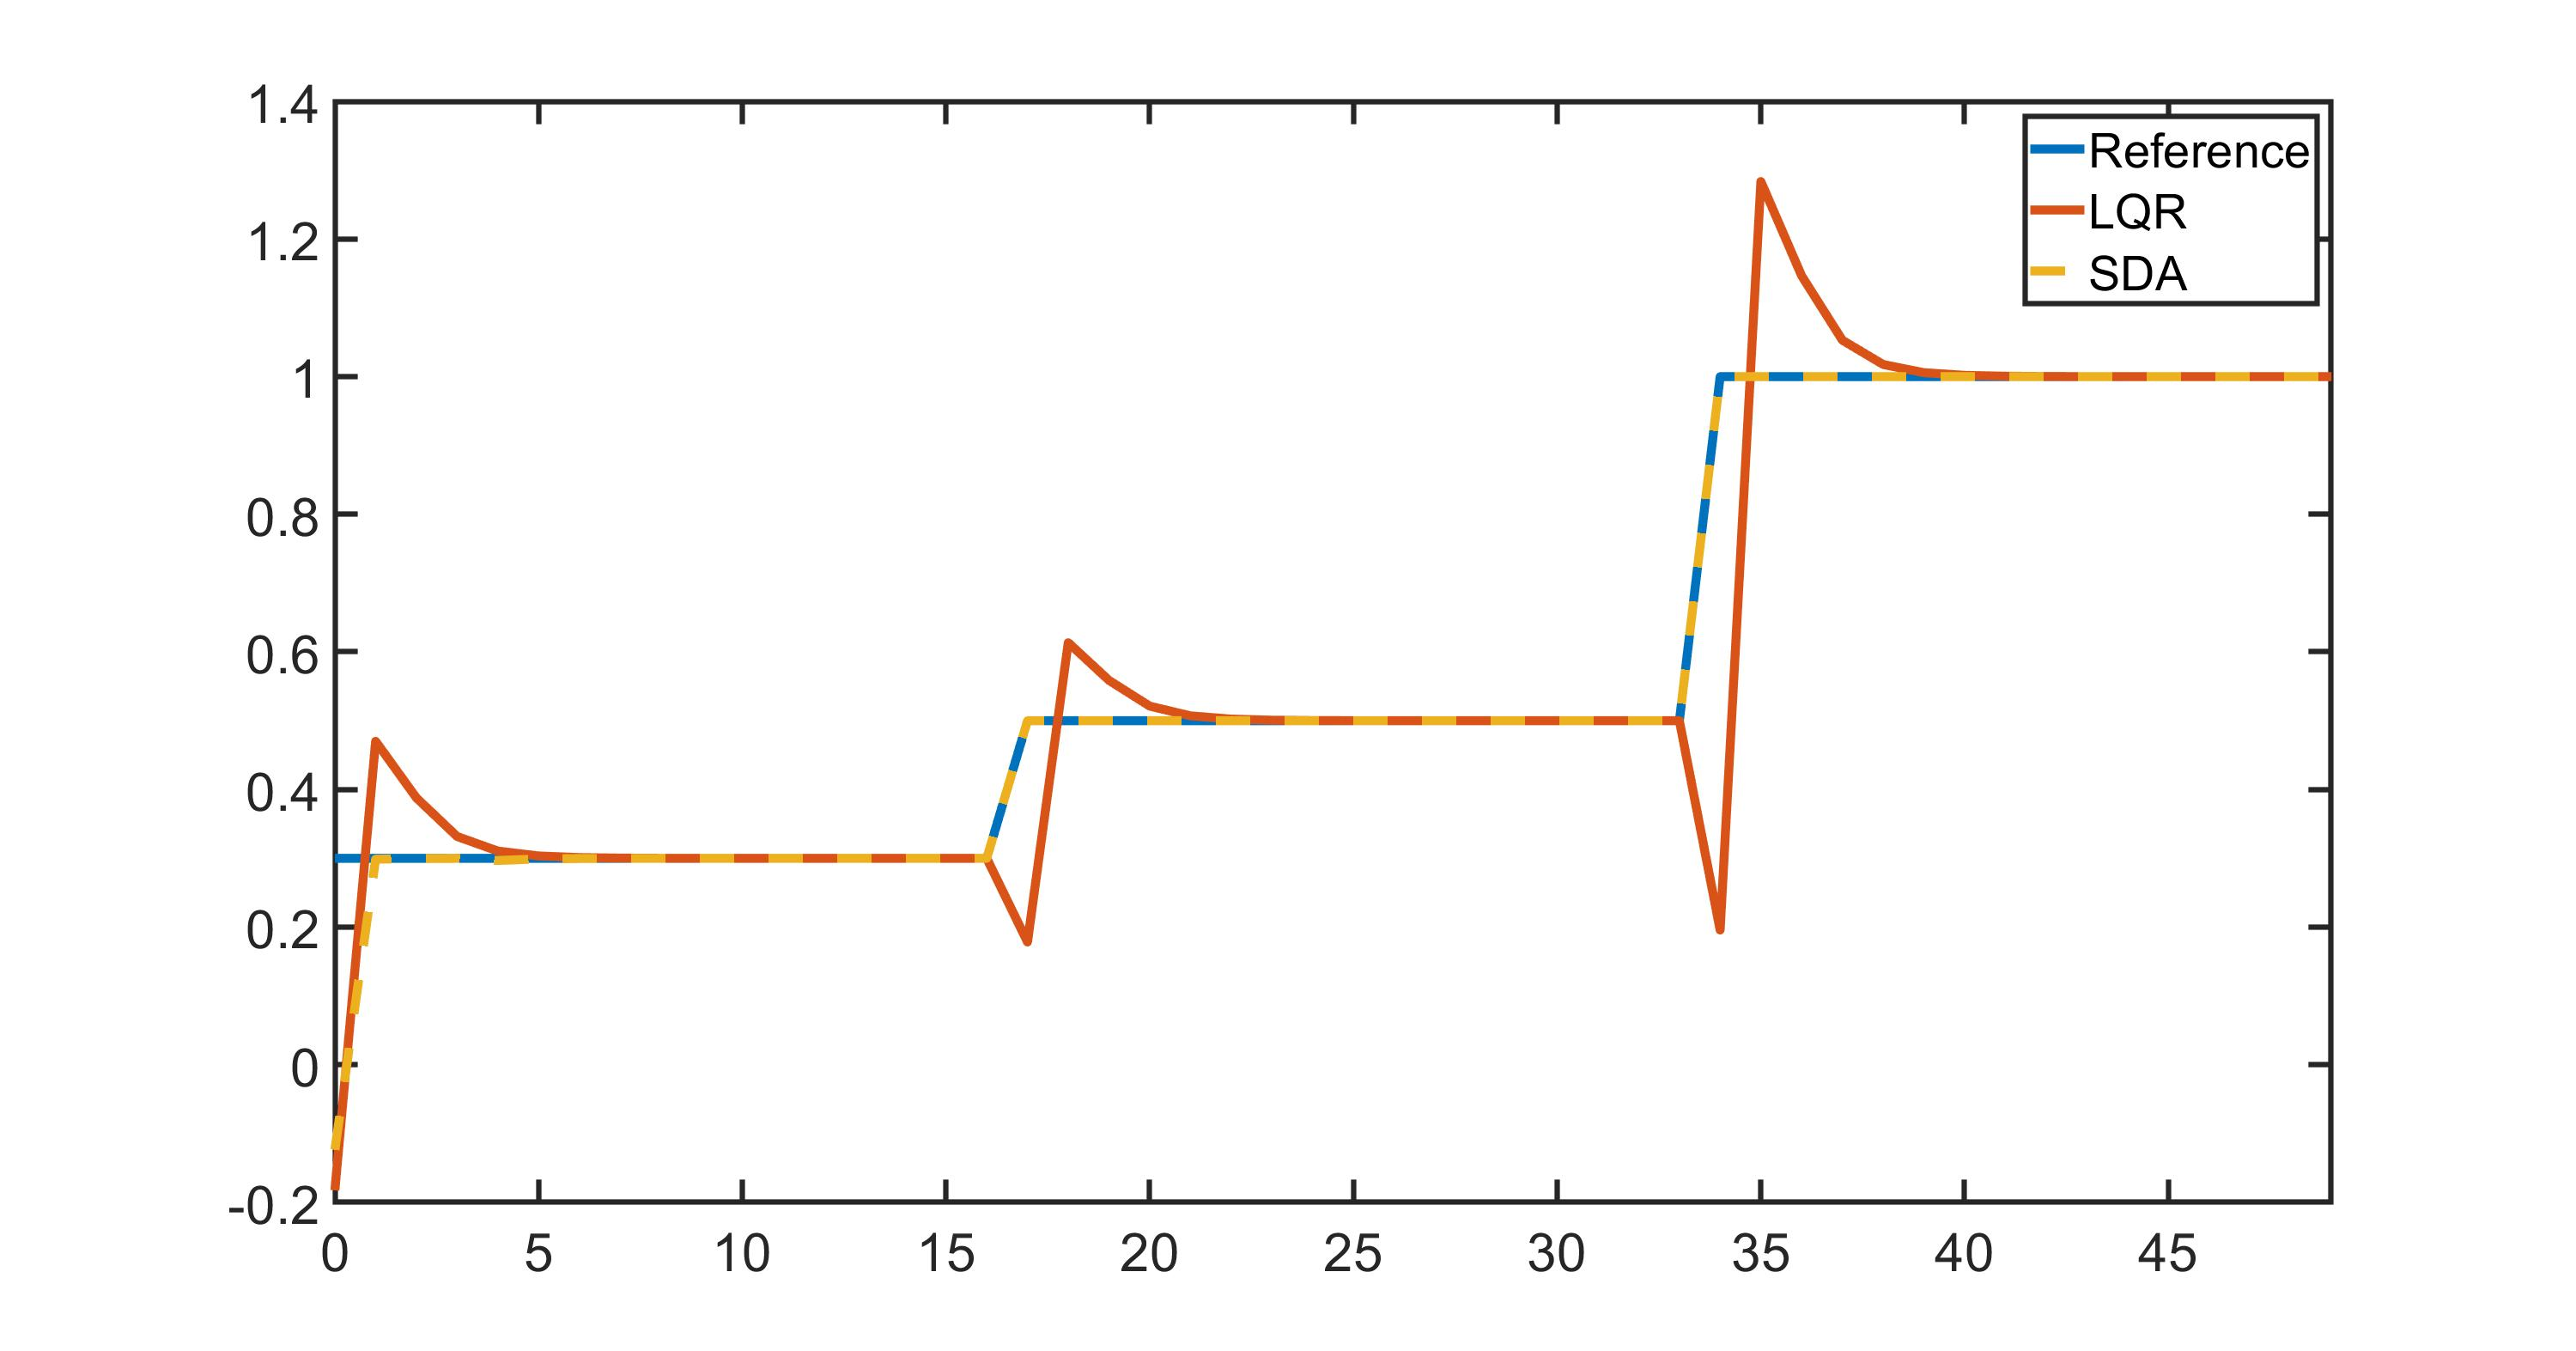
\includegraphics[width=\textwidth]{fig/Ex1_SDA.jpg}
	\caption{Reference signal tracking with SP and SDA for the system \eqref{eq:ILC:Sys_ex1}}
	\label{img:ILC:Ex1_SDA}
\end{figure}

By choosing the weight $R$ we the control action becomes regulated.The limitation of the possible input signals, it also leads to a rapid convergence. For example, for $R = I$ the tolerance of $\tol$ is achieved after 8124 iterations, while with 
\begin{align}
R = \diag \begin{pmatrix}
1& 1 & 1 & 1 & 0.1 & \dots & 0.1
\end{pmatrix}
\end{align}
only 2569 trials are required. 

\end{exam}


\subsection{Suppression of eigenvalues} 

In the previous algorithms the learning matrix $K$ was constant over all iterations. 
Another way is to choose the variable $K_k$ for $k\geq 0$. 

The simplest modification way is to set an iteration varying the gain $\beta$ for each step: $K_k = \beta_k K_0$, $k\geq 0$ for a fixed matrix $K_0$. 
An appropriate choice for $\beta_k$ seems to be the eigenvalues of the matrix $G G^\star$. This motivates the following theorem. 	


\begin{theo}
	Assume, that the matrix $GG^\star$ has $q+1$ non-zero ordered eigenvalues $\lambda_0, \lambda_1, \dots ,  \lambda_q$. Set $\beta_k = \frac{1}{\lambda_k}$ for $k = 0, 1, \dots, \, q$ and consider the update law
	\begin{align}
	\label{eq:cl_var0}
	\begin{split}
	u_{k+1} &= u_k + \beta_k G^\star e_k, \; k \geq 0\\
	u_0 &\in \R^{l (N+1)}.
	\end{split}
	\end{align}
	with error evolution 
	\begin{align}
	e _{k+1} &= (I - \beta_{k+1}  GG^\star) e_{k}  = \prod_{l = 0}^{k+1} (I - \beta_{l}  GG^\star) e_0, \; k\geq 0. 
	\end{align}
	Then the error sequence $(e_k)_{k\geq 0}$ converges in a finite number of iterations.     
\end{theo}
\begin{proof} 
	Set $\t{N} := m(N+1) - 1$. With the spectral theorem, there exists a basis of the eigenvectors $\{v_0, v_1, \dots, v_{\t N}\}$ with corresponding eigenvalues $\lambda_0, \lambda_1, \dots, \lambda_q, 0, \dots 0$. 
	Then $e_0$ can be written as 
	\begin{align}
	e_0 = \sum_{p = 0}^{\t N} \gamma_p v_p
	\end{align}
	with uniquely defined $\gamma_p \in \R$, $p = 0, 1, \dots, \t N$. 
	
	For $k \in \N$ it follows 
	\begin{align}
	e_k = \left(\prod_{j=0}^k(I - \beta_j G G^\star)\right)e_0 = \sum_{p = 0}^{\t N} \gamma_p \left(\prod_{j=0}^k (I - \beta_j \lambda_p I)\right)v_p.
	\end{align}
	
	For the first iteration the error becomes 
	\begin{align}
	e_1 = \sum_{p = 0}^{\t N} \gamma_p ( I - \beta_1 \lambda_p I) v_p = \sum_{p=1}^{\t N } \gamma_p ( I - \beta_1 \lambda_p I) v_p.
	\end{align}
	
	The component $v_0$ is eliminated from the error.
	If for $k \geq 1$ the first $k$ components were eliminated, the $(k+1)$-th error becomes 
	\begin{align}
	e_{k+1} = \sum_{p = 0}^{\t N} \gamma_p \left(\prod_{j=0}^k (I - \beta_j \lambda_p I)\right)v_p = \sum_{p = k + 1}^{\t N} \gamma_p \left(\prod_{j = 0}^k (I - \beta_j \lambda_p I )\right),
	\end{align}
	and hence the first $k+1$ components $v_0, v_1, \dots, v_k$ are eliminated. 
	By induction, the iteration process terminates after, at most,  $m(N+1) - q - 1$ iterations, as all non-zero eigenvalues have been covered and hence all corresponding eigenvectors are eliminated.
		
\end{proof}

Although this algorithm is conceptually interesting, it is not suitable for real-world problems.
The small non-zero eigenvalues of $GG^\star$ will potentially lead to very large values of $\beta_k$ and which follow extremely large transient variations in the error norm. 
%The model errors can make this problem intolerable when elimination of eigenvector components will not be achieved in any iteration and/ or may be re-introduced in later iterations. 

Also computing the eigenvalues can be numerically difficult or deliver not precise results, and hence the eliminating of the eigenvectors is not guaranteed. Moreover, to achieve the monotonic convergence only the eigenvalues $\lambda > \frac{1}{2}\lama(H)$ are an option.
Furthermore, the model inaccuracy or uncertain eigenvalues have direct impact on the algorithm result. 

That all makes this algorithm not solid. Still, the idea to apply the eigenvalues of $G G^{\star}$ still can be used -- but not directly, but by ''picking'' the compatible eigenvalues. 
%TODO: Die Algorithmen umbenennen? Damit es konsistent ist 
\begin{alg}
	Choose a finite number $N_p + 1$ of points $p_0, p_1, \dots$ spread over the half-open interval $(\frac{1}{2}\lama(H), \lama(H)]$. 
	The Gradient Algorithm with Suppression of Eigenvalues (SoEA) is defined via choosing of the iteration-depending control law  $K_k = \beta_k G^\star e_k$, where 
	\begin{align}
	\begin{split}
	\beta_k &= \frac{1}{p_k} \text{ for } k = 0 , 1, \dots , N_p,\\
	\beta_k &= \beta  \text{ for } k > N_p,
	\end{split}
	\end{align}
	with $\beta \in (0, \frac{2}{\lama})$.
	
	Then the input update law becomes 
	\begin{align}
		u_{k+1} &= u_k + \beta_k G^\star e_k, \; k\geq 0,\\
		u_0 &\in \R^{l(N+1)}, 
	\end{align}
	and error evolution results in 
	\begin{align}
	\begin{split}
	e _{k} &= \left[\prod_{l = 0}^k (I - \beta_l  GG^\star) \right] e_{0}, \;  k = 0 , 1, \dots , N_p,\\
	e _{k} &=  (I - \beta GG^\star)^{k - N_p} e_{N_p}, \;  k > N_p.
	\end{split}
	\end{align}	
\end{alg}

This algorithm has the same convergence properties as Algorithm \ref{alg:SDA}, but potentially better convergence rates due to the eigenvalue suppression. Intuitively, the approach will increase the convergence speed in the first $N_p + 1$ iterations, if $N_p$ is large enough for good approximation of the interval $(\frac{1}{2} \lama(H), \lama(H)]$.

\begin{exam}
    Apply SoEA on the system \eqref{eq:ILC:Sys_ex1} with weights $Q = I$, $R = I$.  
	The error evolution we get is illustrated in Figure \ref{img:ILC:Ex1_SDAvsSoE}.
	
	The new algorithm needs only 121 iterations, while for the not adjusted SDA 730 trials are necessary. Indeed, for 31 of 51 eigenvalues $\lambda$ of $G G^\star$ holds 
	\begin{align}
	\lambda > \frac{1}{2}\lama(H) = 461.5 \, .
	\end{align}
	
	Also the influence of the weighting matrices on the convergence speed is here demonstrated. 
	Since no better performance at the first time steps is required, the algorithm converges with much less iterations. 
	   		
	\begin{figure}[ht]
		\centering
		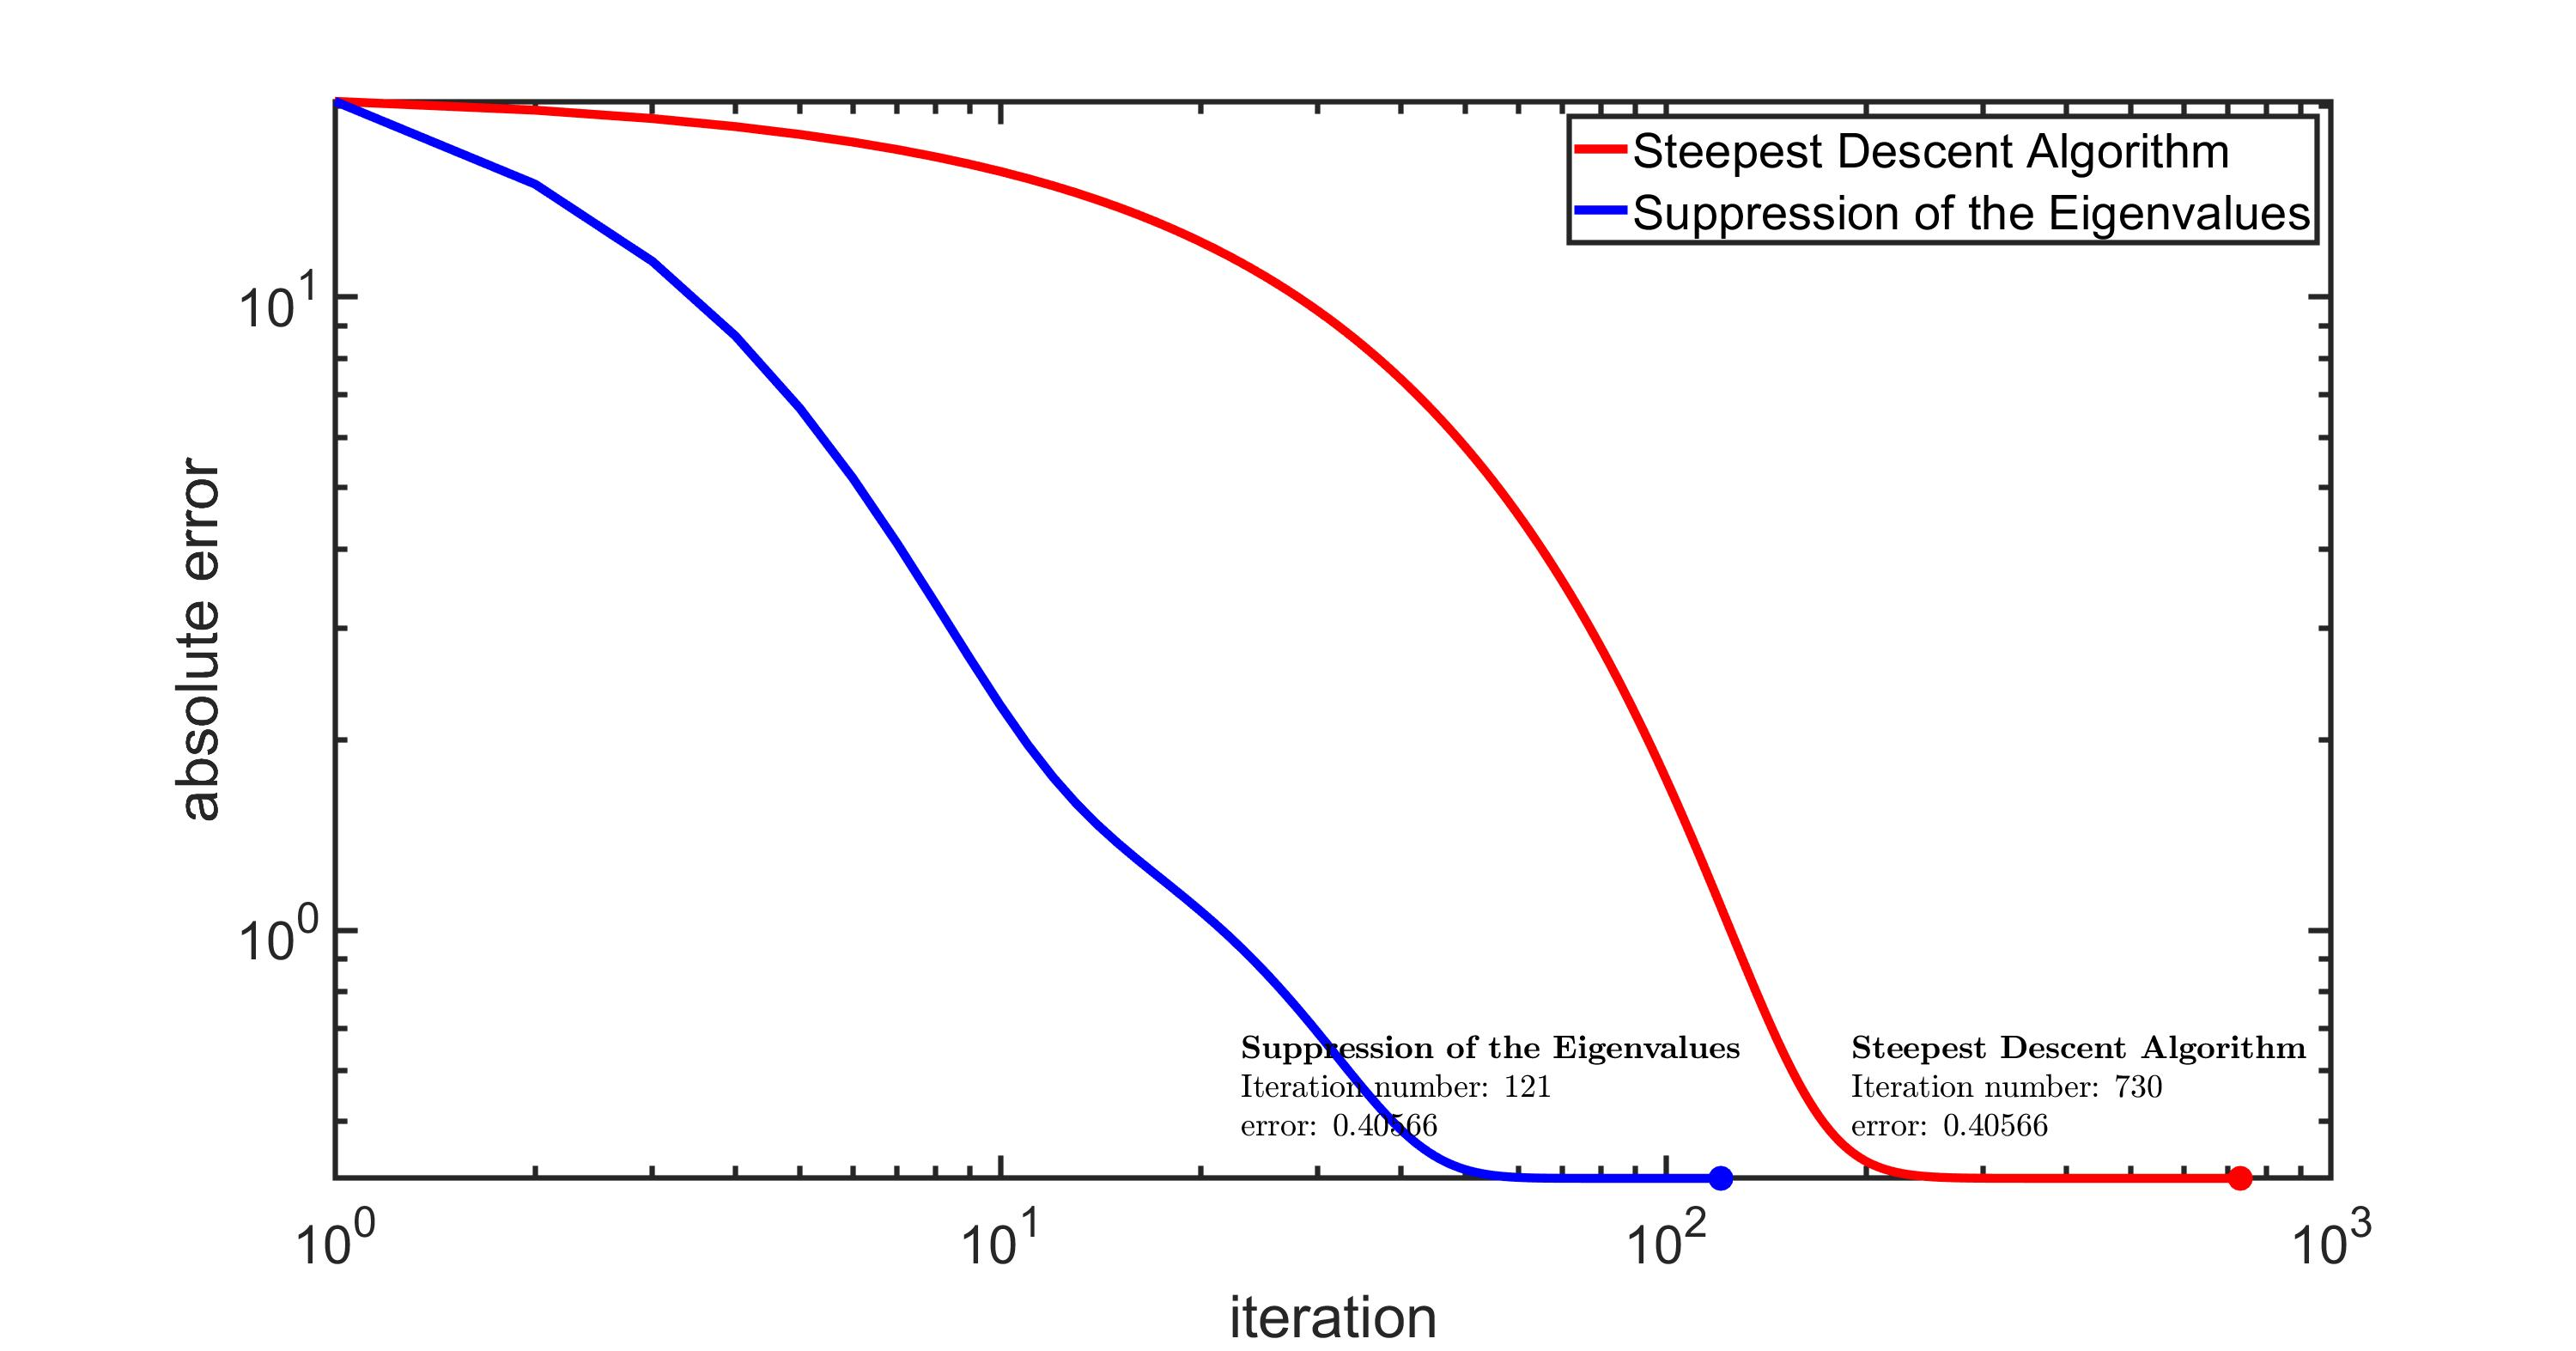
\includegraphics[width=\textwidth]{fig/Ex1_SDAvsSoE.jpg}
		\caption{Error evolution for SDA and SoEA for system \eqref{eq:ILC:Sys_ex1}}
		\label{img:ILC:Ex1_SDAvsSoE}
	\end{figure}
	
\end{exam}

\section{Feedback Design}

The previous algorithms may achieve a better tracking for repetitively executed processes.  But they do not accent the special features of the model. For example, the non-minimum-phase zeros are not managed, but they can impact the convergence rate \cite{ILC}. 
The consideration of the plant structure and contraction of a feedback controller, further converted into a steepest descent-like algorithm can possibly  achieve better performance and robustness properties. 

Denote with $G(z)$ the transfer matrix in variable $z$ of the system $(A,B,C,D)$, and with $G$ the supervector matrix. 

More precisely, consider a forward path compensator $K_c(z)$ in a unity negative feedback system for \eqref{eq:Basics:GP}. 
The design criteria for $K_c(z)$ include the closed-loop stability and the ability to track, albeit approximately, the reference signal $r$. With this compensator, depending on the model, the plant properties such as oscillation, loop interaction, or the effects of non-minimum-phase zeros can be remedied . 

Denote the complementary sensitivity of the resulting closed loop with $T(z)$ and its sensitivity with $S(z)$:
\begin{align}
T(z) = (I + G(z) K_c(z))^{-1}G(z) K_c(z) \text{ and } S(z)  = I - T(z) =  (I + G(z) K_c(z))^{-1}, 
\end{align}
and define the controller
\begin{align}
K_0(z) = K_c(z) S(z). 
\end{align}

Then the compensated Steepest Descent Algorithm is given as follows. 

\begin{alg}
	\label{alg: FBDesign}
	Write the transfer functions in supervector description as 
	$K_0$, $K_c$, $T$ and $S$. The compensated Steepest Descent Algorithm is characterized by choosing  $K = \beta K_0$, $\beta \in \R$. 
	The iterative law is given via 
	\begin{align}
	\label{eq:errFBDesign}
	\begin{split}
	u_{k+1} &= u_k + \beta K_0 T^* e_k, \\
	e_{k+1} &= (I- \beta T T^*) e_{k}, \; k\geq 0,\\
	u_0& \in \R^{l (N+1)}. 
	\end{split}	
	\end{align}
	Monotonic convergence to 
	\begin{align}
	\label{eq:FDErrLim} 
	e_\infty  = \lim_{k\to\infty} e_k = P_{\ker[T^*]}e_0,
	\end{align} 
	is guaranteed if
	\begin{align*}
	0 <\beta < \frac{2}{\lama(T T^*)}.
\end{align*}
$T^*$ stays here for conjugate transpose of the matrix $T$. 
\end{alg}
\begin{proof}
	The proof is identical to that  of Algorithm \ref{alg:SDA} if consider the system
	\begin{align}
	\t y = T\t u + \t d.
	\end{align}
\end{proof}

The effect of the operator $T T^*$ can be seen by regarding the closed-loop relation 
\begin{align}
y = Tr.
\end{align}
A perfect tracking is ensured if $T = I$ -- which is not achievable by feedback control. But still, a good tracking can be expected if $||T|| \approx 1$. 
Therefore if $K_c$ provides excellent feedback control of $G$, then rapid convergence could be attained with a choice of the gain $\beta \approx 1$ \cite{ILC}. % if and the dominant frequency content of the reference $r$ lies in the bandwidth of the closed loop system $T$







%%%% =================================== TRASH ============================================
%Let $(A,B,C,D)$ be a stabilizable system and 
%\begin{align}
%\begin{split}
%&\begin{array}{c c c c c c}
%x_K(t+1) &= &A_K x_K(t)& + &B_K y(t)  &\\
%u ( t) &= &C_K x_K(t)&  + &D_K u_K(t),& \; \; t \geq 0,\\
%x_K(0) &=& x_{K0} \in \R^n & & &
%\end{array}
%\end{split}
%\end{align}
%an according stabilizing controller for this system. Replace the input signal $u$ in the system $(A,B,C,D)$ by a new input $\t u(\cdot) := u(\cdot) + v(\cdot)$ (Figure \ref{img:ILC:stable_cloop}). Then the closed loop interconnection is given via the system 
%\begin{align}
%\label{eq:ILC:stablecloop}
%\begin{mtrx}{c}
%x(t+1) \\ x_K(t+1) \\ \hline y(t)
%\end{mtrx}  = 
%\begin{mtrx}{c | c}
%\t A & \t B \\ \hline \t C & \t D
%\end{mtrx} \begin{mtrx}{c}
%x(t) \\ x_K(t) \\ \hline v(t)
%\end{mtrx}
%\end{align}
%with 
%\begin{subequations}
%	\begin{align}
%	\t A =&\begin{mtrx}{c c}
%	A + B (I - D_K D)^{-1} D_K C & B (I - D_K D)^{-1} C_K 
%	\\
%	B_K C + B_K D (I - D_K D)^{-1} D_K C & A_K + B_K D (I - D_K D)^{-1} C_K
%	\end{mtrx}, 
%	\\
%	\t B =& \begin{mtrx}{c}
%	B (I - D_K D)^{-1} D_K D + B \\ D_K D + B_K 
%	\end{mtrx}, 
%	\\
%	\t C =& \begin{mtrx}{c c}
%	C + D (I - D_K D)^{-1} D_K C & D (I - D_K D)^{-1} C_K
%	\end{mtrx},
%	\\
%	\t D =& D D_K D. 
%	\end{align}
%\end{subequations}
%This new system is stable, and the tracking can still be adjusted using the input signal $v(\cdot)$. 

%\begin{figure}[t]
%	\begin{center}		
%		\tikzstyle{block} = [draw, fill=white, rectangle,
minimum height=3em, minimum width=3cm, align=center]
\tikzset{    sum/.style      = {draw, circle, node distance = 2cm}, % Adder
}

\begin{tikzpicture}[auto, node distance=2cm,>=latex', align=center]
    \node[block](sys){$\left [  \begin{array}{c c}
		A & B \\ C & D 
    	\end{array}\right]$}; 
	\node[block, below = of sys](ctrl){$\left [  \begin{array}{c c}
		A_K & B_K \\ C_K & D_K 
		\end{array}\right]$}; 
	\node[draw, circle, left = 1cm of sys](plus){};
	\node[right = 1cm of sys](phantom){};
	
	\node[draw,dashed,minimum height = 5cm, minimum width = 6.5cm, fit = (sys)(ctrl)(plus)(phantom)](box){}; 
	\node[below = .1cm of box]{Closed loop \eqref{eq:ILC:stablecloop}};

	%y: system output
	\draw[->](sys.0)--($(sys.0) + (1,0)$) node[above]{$y(\cdot)$} -- ($(sys.0) + (1,0)$) -| ($(sys.0) + (1,-1.5)$) -- ($(ctrl.0) + (1,0)$) -- (ctrl.0);
	\draw[->](sys.0) -- ($(sys.0) + (2.2,0)$);
	
	 %u: controller output
	\draw[->](ctrl.180) -- ($(ctrl.180) + (-1.2, 0)$) |- ($(ctrl.180) + (-1.2,1.7)$)node[right]{$u(\cdot)$} -- (plus.270); 

	%input sum
    \draw[->]($(plus.180) + (-2.2, 0)$) -- ($(plus.180) + (-1, 0)$)node[above]{$v(\cdot)$} -- (plus.180);
    \draw[->](plus.0) -- ($(plus.0) + (.5, 0)$)node[above]{$\t u(\cdot)$} -- (sys.180);
    
	
	
	
	
	
	
	
\end{tikzpicture}




%		\caption{Feedback interconnection of the to be controlled system $(A,B,C,D)$ and the controller $(A_K, B_K, C_K, D_K)$, with an extended input $\t u(\cdot) = u(\cdot) + v(\cdot)$. The resulting closed loop system $(\t A, \t B, \t C, \t D)$ is the new stable system used for ILC algorithms, with input $v(\cdot)$ and output $y(\cdot)$} 		\label{img:ILC:stable_cloop}
%	\end{center}
%\end{figure}